\chapter{Adaptive Learning}
\label{chap:adaptive-learning}

% TODO:
% - incorporate other notes from my/thesis gdoc
% - inspiration from relevant articles
% - add references for provided examples (playing chess, autonomous car, ...)

From playing chess to driving an autonomous car,
  artificial intelligence proved to be a mighty tool
  for tackling difficult algorithmic tasks.
The power of artificial intelligence can be also used
  to develop a personalized adaptive system for learning programming.
Such system would create an optimal learning experience for each student
  by providing them with problems of difficulty matching their skill,
  so that the student stays challenged and interested in solving them.

In the existing systems (\ref{sec:existing-systems}),
  the sequence of tasks is the same for everybody.
As a result, the progress is necessarily too slow for some students,
  who could skip some of the tasks,
  while being too fast for others,
  who could highly benefit from solving a couple of other similar tasks.
Artificial intelligence can be used to personalize
  the sequence of tasks for every student.
By giving the student a suitable task
  -- neither too easy, nor too difficult --
  it can help the student to get into the state of flow
  (\ref{sec:motivation.challenge}).

In addition to choosing the most suitable task for given student,
  artificial intelligence has also other possible uses in learning systems,
  for example automatic hints generation \cite{generating-hints}
  or skills visualization (TBA: ref).
Furthermore, artificial intelligence techniques can be used
  to analyze collected data offline.
Such analyses can reveal problematic tasks,
  or suggest how to group tasks into categories (TBA: ref).

Adaptive learning systems have been already successful in some domains.
For instance, Map Outlines%
  \footnote{Available at \url{https://outlinemaps.org}.},
  developed by Adaptive Learning research group at Masaryk University,
  is an intelligent web application for learning geography.
It has been used by tens of thousands of students
  and online experiments have confirmed
  that the adaptivity of the system helps to improve the learning outcome
  \cite{alg.evaluation-geography}.
In addition to geography, similar adaptive web applications
  for learning anatomy%
  \footnote{Available at \url{https://practiceanatomy.com}.},
  biology%
  \footnote{Available at \url{https://poznavackaprirody.cz} (in Czech only).},
  elementary mathematics%
  \footnote{Available at \url{https://matmat.cz} (in Czech only).},
  and Czech grammar%
  \footnote{Available at \url{https://umimecesky.cz} (in Czech only).},
  were developed by the research group in recent years.

Section \ref{sec:student-modeling} presents how to model students
  in the context of learning programming.
Sections \ref{sec:task-recommendation} and \ref{sec:mastery-learning}
  then describe how to use these models to make a learning system adaptive.
Finally, section \ref{sec:metrics-and-evaluation} discusses how to evaluate
  different models or even whole learning systems.


\section{Student Modeling}
\label{sec:student-modeling}

For the system to be adaptive, models of
  a student skill, task difficulty, and student-task interaction
  need to be designed, implemented, and evaluated using collected data.
The purpose of these models is to predict the probability that a given student
  would solve a given task
  and also the time the student would need to complete the task.


\subsection{Data}
\label{sec:student-modeling.data}

To learn model parameters, such as difficulty of individual tasks, some data is needed.
What data and how much data is needed differs across models.
Some data about tasks are independent of students;
therefore, they can be obtained in advance,
which can be useful for initial task difficulties estimates.
Three types of task data are distinguished:

\begin{itemize}
  \item task statement (including name and world description),
  \item sample solution (or multiple solutions),
  \item expert labels (e.g. covered concepts).
\end{itemize}

Task statements are always available,
  because they are needed to present tasks to students.
However, obtaining sample solutions and expert labels
  incurs additional costs for a new system.
% TODO: Note that quite often, systems needs sample solutions and some labels
%       for the presentation purposes anyway.
Moreover, they can be noisy and imperfect.
For example, an annotator can forget to include some labels
  or even make a mistake in the sample solution.

Once the task is deployed in the running system,
  rich data can be collected from each interaction between a student and a task:
\begin{itemize}
  \item whether the task was eventually solved,
  \item solving time,
  \item number of clicks, number of code executions,
  \item program snapshots (e.g. after each code change),
  \item rating or labels provided by the student (e.g. perceived difficulty).
\end{itemize}

% TODO: also consider to include hints in the list
% TODO: mention different granularity levels for taking program snapshots (+cite)

\subsection{Item Response Theory}
\label{sec:irt}

The simplest version of item \emph{item response theory} (IRT)
  \cite{irt-visual-guide}
  models each student by a one-dimension skill $s$,
  and each task by a one-dimension difficulty $d$.
IRT assumes that the probability of a student with skill $s$
  successfully solving a task with difficulty $d$
  is given by the following function:
  \begin{equation}\label{eq:logistic}
  P(s, d) = \frac{1}{1 + e^{-(s - d)}}
  \end{equation}

% TODO: mention 2-parameter model (explain discrimination parameter)
\begin{figure}[h]
  \centering
  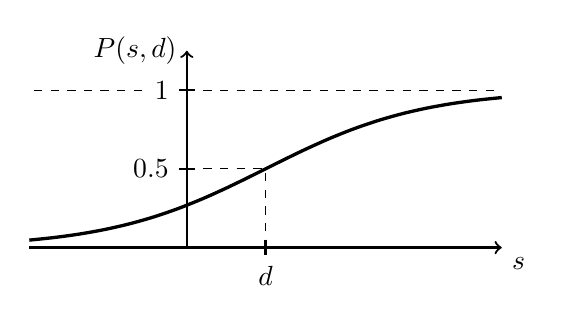
\begin{tikzpicture}[domain=-2:4, smooth, samples=20, scale=1]
  \draw [thick, ->] (-2,0) -- (4,0) node [below right] {$s$};
  \draw [thick, ->] (0,0) -- (0,2.5) node [left] {$P(s,d)$};
  \draw [thick] (-0.1,1) node [left] {$0.5$} -- (0.1,1);
  \draw [thick] (-0.1,2) node [left] {$1$} -- (0.1,2);
  \draw [thin, dashed] (0,2) -- (4,2);
  \draw [thin, dashed] (0,1) -- (1,1) -- (1, 0);
  \draw [thin, dashed] (-0.57,2) -- (-2,2);
  \draw [thick] (1,0.1) -- (1,-0.1) node [below] {$d$};
  \draw [very thick] plot (\x, {2 / (1 + exp(1 - \x))});
  \end{tikzpicture}
  \caption{One-parameter Unidimensional Logistic Model}
  \label{fig:logistic-model}
\end{figure}

This basic model was originally developed for a simple knowledge testing
  and therefore it assumes a single constant skill.
However, programming skill is multidimensional;
  for example, one student can be proficient with functions and struggle with loops,
  while another student can master loops and struggle with functions.
Furthermore, these skills should be ideally changing significantly during
  the interaction with the system, because students are learning.

Another drawback of the IRT is that it only uses
  the binary data about successes and failures.
As nearly all interactions in programming learning systems end with a solved task,
  it would be more useful to work with solving times,
  which can provide more information about students' skills.

Item response theory can be extended to overcome these limitations.
\emph{Problem Response Theory} (PRT)
\cite{alg.problem-response-theory, pelanek-student-modeling-times}
% TODO: only cite the more relevant paper (or extend this section and cite both
% on relevant places)
predicts problem solving times instead of probability of success,
assuming an exponential relationship between a problem solving skill
and the time to solve a problem.
PRT can be formulated to use multidimensional skills.
The model parameters (skills and difficulties) can can be estimated from the data
  using one of the \emph{maximum likelihood estimation} algorithms.
  % TODO: cite paper describing the parameters estimation (or MLE?)
% (for IRT, it's \cite{irt-theory-and-practice}, but PRT would be better)

% TODO: find and provide the details about the learning extension of PRT
% (isn't it already the elo?)

% TODO: Add note that the assumption of exponential relationship is justified
% by observed solving solving times distribution and it is also intuitively
  % plausible - multiplicative nature of solving times.



\subsection{Elo}
\label{sec:elo}

The Elo model \cite{alg.elo}
  extends the logistic model presented in section \ref{sec:irt}
  to capture changing knowledge.
Inspired by the rating of chess players \cite{elo-rating},
  the model interprets each attempt  to solve a task
  as a ``match'' between the student and the task.
After this match ends, skill and difficulty estimates are revised.

If the student solves the task faster than expected by the model,
  their skill is increased and the difficulty estimate of the solved task is decreased.
On the contrary, if the student fails to solve the task or if takes them too long,
  their skill is decreased and the difficulty estimate of this task is increased.

% TODO: formulas (for time-variant of elo)
% TODO: mention differnet updates for tasks (exponentially decayed) and
% students (their skill is assumed to change and not converge)

The main advantage of using the Elo model is its simplicity, flexibility,
  good performance and intrinsic online nature, which allows for immediate
  updates of parameters as students are interacting with the system.

% TODO: include other models, PFA, BKT etc.


\subsection{Concepts}

% TODO: consider to move this section before the description of individual
% models
% TODO: fix and mention used terminology: concept vs. skill

A vast amount of research in the field of adaptive learning
  restricts its attention to a one-dimensional skill.
This assumption is reasonable for many logic puzzles (e.g. sudoku);
however, solving programming tasks requires multiple diverse skills,
  such as loops, conditional commands, or functions.
It is possible to master loops while struggling with functions,
  and vice versa.

As mentioned in sections \ref{sec:irt} and \ref{sec:elo},
  both the IRT and Elo models can be extended to work with multidimensional skills.
% TODO: However, the way they compose multiple skills into a single prediction
% is not completely justified / can differ depending on domain/skills (e.g.
% adding skills vs taking best/worse)
Although modeling multiple skills seems useful,
  there is a trade-off between the complexity of the model (number of skills)
  and how well (or how fast) the parameters can be estimated.
More parameters require more data and time for the estimates to converge.
% TODO: which is especially concern for students; 1. predictions needed
% immediately for new students (no/little data), 2. students' skills are
% assumed to change (tasks didn't have these problems)


% \subsection{Learning Concepts from Data}

Concepts can be either defined manually or detected automatically
  \cite{niznan-thesis}.  % TODO: specify chapter/pages
Manually selected concepts, such as loops and conditional commands,
  have the advantage of being interpretable,
  so they can be used for skills visualizations in the user interface
  to provide students with the information about their learning progress.
Furthermore, no data needs to be collected in advance,
  while the automatic techniques require a lot of data to provide stable results.  % TODO: how much?


% \subsection{Prerequisites}
Undoubtedly, there are some relationships between skills;
  for example, nested loops cannot be mastered without mastering simple loops.
The hierarchical structure between concepts can be modeled
  as a directed acyclic graph (DAG),
  where each vertex is a concept and each edge represents a prerequisite.
Having DAG of concepts then allows to model students using Bayes networks
  \cite{its-programming}.

% TODO: simple diagram: DAG of concepts example

\section{Task Recommendation}
\label{sec:task-recommendation}

Student models are used by an \emph{instructional policy} to recommend
  the most suitable task for a student.
In spite of having all the predictions about success probabilities
  and time estimates available,
  task recommendation is not an easy task.
First, it is not clear what difficulty level is optimal.  % TODO: example (75 % of success etc.)
Second, it may vary for different students, domains or types of problems.
Furthermore, optimal difficulty is not the only criterion to be considered.
For instance, diversity of tasks is important to keep students interested.
No principled techniques for task recommendation have been developed yet;
however, several heuristic approaches have been used
  and proved to work well (TBA: ref).

Task recommendation is not a necessary requirement
  for the system to be adaptive.
Student models can be utilized by other means to achieve personalized behavior,
  e.g. in mastery learning (section \ref{sec:mastery-learning}).
The system can also just provide students with predicted solving times
  and let them to choose the next task they want to solve.

Showing predictions can be already perceived as a very mild form of recommendation.
Indeed, recommendations can range from \emph{soft} to \emph{hard}.
Soft recommendations can be achieved either by
  ordering tasks according to suitability,
  filtering and only showing a subset of tasks,
  or showing suggestion such as
  ``too easy'', ``too difficult'' and ''ready to attempt'' next to each task.
For example, suggestions in the form of traffic-light colors
  are used in the system described in \cite{its-programming}.
The system can be more strict and show only a single recommended task,
  or even enforce the recommendation by immediately progressing student to
  the next task without asking and giving them a chance to select a different task.

\bigskip
\emph{TODO:\\details about techniques (heuristics, methods) for selecting single best task}

% TODO: mention simple heuristic approach from Tutor: 2 tasks of similar difficulty as the just solved task which were not solved previously

\section{Mastery Learning}
\label{sec:mastery-learning}

\emph{TODO:\\describe mastery learning + usage of student models%
(to show the progress and to determine that the student already achieved the mastery)}

% "fixed outcome, varied time" (vs. classical education: fixed time, varied outcome)

% TODO: screenshot of a mastery progress bar (e.g. from UmimeX)

\section{Metrics and Evaluation}
\label{sec:metrics-and-evaluation}


To decide if the adaptivity improves the quality of the learning system,
  a suitable metrics must be chosen and evaluated.
Metrics are also used for optimizing models,
  first for parameters fitting, second for choosing hyperparameters
  and third for selecting best possible model from a set of possible models.

%TODO: table/diagram showing goals hierarchy and their usage:
%1. mission -> guide for long term objectives? (not measurable)
%2. long term objectives -> AB experiments
%3. live evaluation
%4. offline evalution
%5. etc.

\subsection{Mission Statement}
\label{sec:mission}

There are hundreds of possible metrics that the system could measure.
What metric to choose depends on the purpose of the evaluation,
  which can range from guiding a parameters-fitting algorithm
  to interpreting results of an AB experiment.
To make sure that chosen metrics are not misleading,
  they should reflect the ultimate goal of the system,
  which is sometimes also called \emph{mission}.

Even the mission itself should reflect some higher-level goals.
Nevertheless, goals create an infinite hierarchy
  and a starting point (called \emph{paradigm}) must be chosen from which
  the lower-level goals are derived.
An example of such paradigm is
  ,,effort to maximize the overall happiness in the population''.
% TODO: Without going into further philosophical discussions or attempts for precise definitions,
%       ... we will just adopt this paradigm for the rest of this thesis.

At first sight, a reasonable mission of a system for learning programming
  is a long-term increase in algorithmic-problem solving skill in the population.
However, other factors than skill should be considered as well.
For example, how much students enjoyed the time in the system,
  how they are satisfied with their accomplishments,
  or if they are motivated for further learning of programming;
  all of these may play an important role for the overall happiness in the population.
In the \emph{Rules of Machine Learning}, Martin Zinkevich
  points out that there is no single best objective \cite[][Rule \#39]{google-ml-rules}.
As a solution to this ,,multiple objectives dilemma'',
  the mission can be formulated as achieving a balanced increase in all
  of these important factors.
Such formulation helps to remind developers of the system not not overfocus on one factor
  in the cost of the others factors.


\subsection{Long Term Objectives}
\label{sec:long-term-objectives}

The huge disadvantage of the mission statements
  is the fact that they are not measurable.
To make informed decisions,
  such as which of the two recommendation algorithms to prefer,
  measurable metrics are needed.
Therefore, various proxy metrics are used,
  which should be precisely formulated and measurable,
  but at the same time they should be related as much as possible to the system mission.

To elaborate on the mission from section \ref{sec:mission},
  a long term objective could be
  ,,maximizing the number of students
  who mastered elementary programming quickly while having fun''.
To make this metric usable,
  terms ,,mastering elementary programming'', ,,quickly'', and ,,having fun''
  must be defined in a measurable way.
While ,,achieving mastery in elementary programming quickly'' can be
  formulated as an objective criterion
  (e.g. ,,the student solved at least 5 tasks for each concept, each in less than 5 minutes''),
  ,,having fun'' requires the system to ask students about their subjective feelings.
% TODO: note that looking at the mission statement above,
% it's not clear that there must be an objective mastery criterion
% which should be achieved by all students

Furthermore, a time frame must be specified
  -- usually a few weeks for AB experiments.
While short time frames allows for faster decisions and hence more improvements over time,
there are several reasons for making the time frame longer:
\begin{itemize}
  \item to collect enough data for statistical significant results,
  \item to avoid seasonality effects (such as different user behavior during weekends),
  \item to allow the system for more exploration, which improves long-term performance of the system.
\end{itemize}

Instead of a fixed length time frame
  it is also possible to formulate the metric as
  an infinite sum over all future time moments.
To make sure the infinite sum converges
  the values in the sum must be carefully weighted with respect to time.
  % TODO: elaborate
  % + this also makes it possible to compute the min-max interval at any given time


% TODO Some other examples:
% TODO (consider): add "Maximizing XY" to all metrics below
%\begin{enumerate}
%  \item Sum of exponentially-time-decayed flow-minutes. (TODO: explain)
%  \item TBA
%\end{enumerate}

%In the case of flow-minutes, one way is to ask students for the perceived flow.
%Alternatively, the metric can be proxied further to obtain a one
%  which is more easily measured,
%  e.g. number of minutes spent by solving task which end with successfully solved task.

\subsection{Live Evaluation}

In some learning systems, a new version of a model is deployed every day
  with parameters learned from the recent data.
The behavior of the new model must be carefully monitored
  to detect problems as soon as possible,
  without waiting several weeks to evaluate an AB experiment.
For this purpose, metrics that can be linked immediately
  to the recommender actions are needed.
These metrics are called ,,online attributable metrics''  % TODO: find used terminology
and this type of evaluation ,,live evaluation''.

These metrics are often formulated as a question concerning a single recommendation.
To transform them into a number, either sum or average of these individual errors is computed.
% TODO: so sum or average? or some other aggregation function?

Reflecting the long-term objectives from section \ref{sec:long-term-objectives},
  there are some examples of online attributable metrics:
\begin{itemize}
  \item Was the recommended task chosen by the student?
  \item \ldots and did the student solved the task?
  \item \ldots and in a reasonable time (e.g. 1-15 minutes)?
  \item \ldots and did not the student marked it as ,,too easy'' or ,,too difficult''?
\end{itemize}


% TODO: note on online models (and relation to RL), these needs continuous online evaluation

% TODO: taking delta wrt. previous model


\subsection{Offline Evaluation}

Offline experiments use historical collected data
  to avoid the cost of live evaluation.
The advantages of offline experiments compared to online evaluation include
  the possibility to run as many experiments as needed,
  obtaining the results quickly,
  reusing the same data to evaluating different models,
  and avoiding potential negative impact on students if the evaluated model is poor.

Of course, the offline evaluation is limited,
  because there are not all the historical data needed
  for proper evaluation.
For example, when evaluating a new recommendation algorithm
  the data on how the student would respond to a particular recommendation
  are often not available.
% TODO: mention another limitation - the population is changing
% TODO: note: further decrease of relevance to the system mission - but worth

Offline evaluation is typically used as a check before pushing
  the model online to avoid problems as soon as possible.
It can be also used for model selection,
  including hyperparameters search.
Finally, offline learning algorithms typically also use
  a metric to guide them
  (these are discussed in section \label{sec:metrics-to-guide-learning}).

\subsection{Cross Validation}

\emph{TODO}


\subsection{Evaluating Student Model}

Student models (described in \ref{sec:student-modeling})
  are important subcomponent of techniques for adaptive learning,
  such as recommendation algorithms.
Therefore it is reasonable to believe that optimizing the quality
  of used student models should result in better recommendations
  and transitively in improving the long-term objectives.
However, this relationship is not as simple
  and improvements in the predictive power are not worth
  if the online experiments show that they actually
  decreased the long-term objectives.

The next two sections present metrics for two most common
  types of student models according to their output:
  predicted solving times and predicted success.
% TODO (consider): generalize: any real values (e.g. times)
%                  vs probabilities (success, too-difficult)

\subsection{Metrics for Time Predictions}
\label{sec:metrics-for-time-predictions}

% TBA: note on data we need (and easily collect in this case)
To evaluate the quality of solving times predictions,
  vector of predicted times $\hat{t}$ is compared to
  the vector of true observed times $t$.
Usually, individual errors between tuples $(t_i, \hat{t}_i)$ are computed
  and then averaged.
While it is possible to take an absolute value of the
  difference $(t_i - \hat{t}_i)$,
  which results in Mean Absolute Error (MAE),
it is more common to taking square of the difference
  to penalize more one large error than multiple small ones.
In this case, it is common to take a square root of the final
  average, to bring the units back to the original ones
  for better interpretation.
This metric is called Root Mean Squared Error (RMSE).

$$
RMSE(t, \hat{t}) = \sqrt{\frac{1}{n} \sum_{i=1}^n (t_i - \hat{t}_i)^2}
$$

Note that the solving times are should be first log-transformed;
  otherwise a single outlier could make the error extremely high.
% TODO: provide more details/ref to an earlier section about taking logs
% TODO: also note that these type of metrics will be always susceptible to
% outliers anyway

% TODO: Statistic notes why the RMSE makes sense:
%       - explain that given some assumption
%       -> results in best linear estimator
%       - and even MLE (assumption of normally distributed noise),
%                       -> it's equivalent to RMSE - see Bishop, 2006)

%TODO: The metrics presented in this section
%  can be also used for evaluation of other real-valued predicted variables,
%  such as flow (if formalized to take real values.)


\subsection{Metrics for Success Predictions}

Some student models predicts a probability that
  a given student will solve a given task.
% TODO: statistics terminology - alternative distribution
In this case, each the true labels are not any real number,
  but just zeros and ones.
This difference is important for the choice of a suitable metric.
Good overview of possible metrics is presented in \cite{pelanek-evaluation-student-models},
  which also shows a simple example demonstrating why MAE should not be used
  as an error measure for binary predictions.
In addition to RMSE, Log-Likelihood (LL) is sometimes used:
$$
LL(s, \hat{s}) = \sum_{i=1}^n s_i\log(\hat{s}_i) + (1-s_i)\log(1-\hat{s}_i)
$$
% TODO: include derivation of LL from MLE principle (product -> log -> sum)
Note that LL differs from RMSE in several aspects.
First, as opposed RMSE, the higher LL the better,
second, it is negative,
and third, it is not averaged, so it decreases with the size of data set.

The RMSE and LL are based on a probabilistic view of errors.
There is another set of metrics based on the qualitative understanding of errors,
  which compares the observed success with binarized predictions,
  instead of real-valued probabilities.
For example, \emph{accuracy} is a ratio between correct predictions to all predictions.
However, these metrics do not distinguish between small and large errors of the predictions,
  which makes them less appropriate for student modelling.

% TODO: details, possibly table of common metrics from the confusion matrix
% (precision, recall, sensitivity, specificity, ...)
% TODO: mention: allows for setting different risks (weights) on different types of errors
% TODO: diagram: comparison of these individual errors, see pelanek-evaluation-student-models, p.6

These error metrics depends on a particular threshold chosen
  for binarization of predicted probabilities.
There are metrics avoiding this problem byt using only ranking of predictions.
The most common one is AUC -- ,,Area Under Curve'',
  which is the probability that if one failure and one success are selected by random,
  the predictor would assign a higher probability to the success event than to the failure.

There are a few limitation of AUC.
First, it considers all thresholds, but only a range of them is usually relevant.
Second, by only considering the ordering of predictions,
  if all predictions are multiplied by a constant, AUC remains unchanged.
Third, if the predicted classes are strongly unbalanced, AUC of nearly 1
  can be achieved by a simple baseline predicting the majority class.
Generally, AUC is a reasonable choice for intrinsically classification problems,
  but not for student modeling \cite{pelanek-evaluation-student-models}.

% TODO: precise definition of AUC using ROC curve
% TODO: check if the intuitive explanation of AUC is correct
% TODO: how to deal with the limitations: global objectives (ranges of thresholds), AUC-PR for unbalanced problems


\subsection{Metrics to Guide Learning}
\label{sec:metrics-to-guide-learning}

\emph{TODO}

% aaah! both online and offline - how does it fit to the hierarchy?
% examples
% - LL to guide logistic regression
% - (RMSE for linear model predicting solving times),


\subsection{Simulation Experiments}

Online experiments relies on live data,
while offline experiments use historical data.
Simulated experiments provide a third alternative,
  which does not require any collected data at all.

Not needing collected data makes simulations widely and easily applicable.
On the other hand, researchers must be careful when interpreting
  the results of a simulation, as the simulation results are noting more than
  just consequences of used assumptions.
Nevertheless, simulation are perfect for models debugging,
  for example to find fatal errors in the implementation.
Furthermore, \emph{sensitivity analysis} is a technique to find
  which parameters of the model are important and should be learned,
  and which can be safely set manually without frequent retraining.

In practice, simulations can also take advantage of collected data
  if they are available; to estimate some of the model parameters
  or to evaluate how much the model predictions agree with
  what was observed in the reality.






% -------------------------------------------------
% -------------------------------------------------
% -------------------------------------------------
% -------------------------------------------------
% -------------------------------------------------
% -------------------------------------------------
% -------------------------------------------------
% -------------------------------------------------
% -------------------------------------------------
% -------------------------------------------------
% -------------------------------------------------
% -------------------------------------------------
% -------------------------------------------------


% \subsection{Metrics for Predictions}

% compared to other RS, evalution is more difficult,
  % - what we care about (= learning) is what is in student's head
  % (note on behavioral vs. cognitive view?)
  % -> only indirect measures (proxies)

% terminology:
  % - metric = function from the space of models to real numbers (note that it's different from the mathematical "metric" which assigns a number to a pair of objects and must satisfy some properties) (also needs to specify the desired direction to be useful..)
  % - objective = a metric which is optimized by an algorithm (often: we monitor multiple metrics, but only optize a single metric by a single algorithm; reasons for not opitmizing a metric: difficult/infeasible to optize, or we are not sure if this is actually what we want to optimize)


%TODO: data we need -- this is simple: we can collect the objective solving times and compare
%with predictions (there is some noise, because of students taking breaks, cheating, etc., but should be ok)

% methodology: Train-Test split of collected data
% -> train on train-set -> predict for test-set -> compare
% - K-fold cross-validation - on students ok ("user stratified"), but:
% - make sure to predict future from the past
% - REF: details in Radek's paper on student models



% sometimes, these metrics are directly used as an objective during parameters fitting
% (examples: OLS minimizing MSE, logistic regression minimizing log-likelihood ?)


\subsection{Metrics for Recommendation}

\emph{TODO}

% good predictions are important, but at the end we care about the performance on some other task,
% for example recommendation -> need to measure performance of recommendation
% + don't apply changes improving predictions if they degrade performance on recommendation

%TODO: what data to use? much less clear than  for predictions
% - manual labelling? (what task should be recommended to this student) -> very demanding (and probably error-prone)
% - historical - collected data: con: only for the task we actually recommended (for this we can say, if the student has clicked on the recommendation and solved the task in a reasonable time)
% - process: train-test split (with past-future consideration)
%   -> train recommender on the train-set -> compare to the actual actions
%   (e.g. did the student selected/solved the task we recommended to them)
%   - drawback: student usually select the task which was recomended to them,
%     that doesn't mean it was good and that they would choose it themselves
%   ( -> can limit our data only to cases where the student decided themself x just another data bias?)

%TODO: mention standard metrics and evaluation methodologies in RC (for recommended tasks)
%
%The tasks environment in learning systems often differ significantly
%  from the real-world environment,
%  e.g by using blocks instead of text
%  and other aspects mentioned in section \ref{sec:strategies-for-easier-learning}.
%This makes evaluation harder, because while the collected data on which we
%  evaluate the system comes from the system itself,
%  ultimately students leave this simplified environment
%  and the performance outside the learning system is the important criterion.

% This issue is mentioned in \cite{challenges-of-blocks-based-environments},
% by Werntrop and Wilensky
% in the context of proper evaluation of block-base programming environments.

% TODO: this relates to next subsection on ultimate goal vs. proxy metrics
% TODO: also consider short discussion on high-level vs. low-level goals
% (also known as mission/purpose/vision vs goals, or goals vs means
% and discussion on goals vs metrics


% mention ranking metrics, such as topK
% - why: frist places are important, the last are not (because only the items on first places get recommended)
% - ranking metrics: Spearman correlation coefficient, half-life utitily, liftindex, discounted cumulative gain, average precision (sounds similar to AUC-PR...?)


% important properties x but harder to measure than simple accuracy:
% e.g: confidence, diversity, utility, robustness
% explain why: e.g. diversity - if we show multiple recommended tasks, they should be diverse, otherise we could have shown just one (+ diverse from the previous task ... in case the student solved the last task withou a problem) --> our current item-similarity research


% - for binary/binarized predictions: accuracy, precision (precision@n), recall, F1 (harmonic mean of precision and recall), confusion matrix


\subsection{Feedback Loops}

\emph{TODO}

% big issue in recommendation systems in general
% TBA: give an examle (including the resulting problem)
%   - we only collect data on what we recommend -> bias
% REF: Google Rules of ML 36


%\subsection{Ultimate and Proxy Metrics}
%
%\emph{TODO}

%TODO: explain possible metrics derivation: -- with specific example of learning programming
%1. from the ultimate goal (vision, mission, purpose, ultimate objective) -- but make it precise to make it evaluable (if had all the data we need)
%2. proxing 1 to make it measurable in the long term (AB experiment)
%3. proxing 2 to make it measurable in the short term (live evaluation)
%4. proxing 3 to make it work with offline data (to learn hyperparameters + for holdout evaluation)
%5. proxing 4 to make it differentiable function (to guide learning, ie. for updates after new s-t interaction)

% Long-term live evaluation (for AB experiments - or just as reporting metrics)
% - can be indirect as popposed to the immediate-evalution, ie. measuring aggregate effect of
%   all recommendations during the period
% - number of students who solved at least 10 tasks from the final level
%   (or at least one from each level)
% - total number of credits earned? (not well-defined unit)
% - daily/monthly number of students /  number of students solving at least one task
%   (terminology DAU = 1 day active users, 30DAU)
% - daily number of solved tasks (-> would lead to recommendation of short tasks)
% - total time spent on our site by all students (-> but we want them to practice not just be on our site)
% - total time spent by solving tasks (-> but we want them to learn quickly?)
% - total time spent in flow (requires measuring/proxying flow)
% - direct: number/ratio of times the recommendation button was clicked
%   + and followed by a succesfully solved task
%   + and not marked as too-easy/difficult/boring/weird
% - proportion of returning students (?)


% Online experiemnts -> AB testing
% -> randomized control trial
% -> diagram of A/B testing, e.g. https://receiptful.com/blog/ab-testing-for-ecommerce
% - needs a metric for comparison
% - there will be always a differnce -> needs to asses statistical significance
% (is the difference due to changed condition or just because of random noise)
% -> t-test and similar (but mind their assumpations!) -> p-value + alpha-level -> decision
% -> add error bars to measured metrics: e.g. 95% confidence interval / standard eror / standard deviation / range
% (+ effect size)


% Multiple objectives dilemma (the one we will directly optimize):
% - not so important when deploying a new ML system:
% - REF Google Rules of ML, rule 12: "Don’t overthink which objective you choose to directly optimize. (...) early in the machine learning process, you will notice them all going up, even those that you do not directly optimize."
% (example: we might care about daily number of students who solved at least 1 task, or total number of tasks solved during a day, or total number of clicks on our site etc. Optimizing one of them will most likely lead to optimizing the others as well, at least at the beginning - all relavant metrics will go up)
% Rule 13: "Choose a simple, observable and attributable metric for your first objective."

% enjoyment vs. learning metric
% - enjoyment is easier to measure (length of interaction), but is not we we ultimatelly care about
% (maximizing would lead to pure enjoyment without learning)
% - and pure learning is also not enough, because intensive learning is not worth if the students lose interest and leave the site --> need for balance (as always...) ("principle of balance")
% measuring enjoyment -> survival analysis
% measuring learning
% -> learning curves
% - pretests and postests
% - or only postests (to compare different models, AB experiment)

% live evaluation:
% - important
% - issue: population shift (violation of the same train-test distribution assumption)


% Danger: proxy metrics vs."the ultimate health of the system"
% see Goole Rules of ML, rule 39


%\subsection{Perceived Flow}
%
%\emph{TODO}

%Instead of using objective ("quantitative", "factual", "measured") data (such as solving time),
%we can ask students to provide explicit ``rating'' ("qualitative","subjective") (e.g. perceived difficulty),
%  e.g. by selecting tags after solving a task,
%  such as ``too easy'', ``too difficult'', `just right''
%  (or possibly even more specific such as ``boring'', ``weird'', ``fun'').
%Advantage: flow looks as a good proxy metric to optimize.
%Disadvantages:
%  bother students with another questions,
%  takes time (but this is negligible comparing to solving programming task),
%  inaccurate (noise depending on the mood etc.)
%

% Other qunatitative feedback: free feedback (via feedbck button or form, talking to people after formal/informal user testing) - extremelly useful as well (TODO: give some examples)

% flow:
% - principel of balance: in the real life, many things (maybe all) are about
%   finind a balance, not about maximizing/minimazing something -> flow is a
%   good demonstration of this principal
% - not tangible (needs some units and precise definition?)
% - set e.g. 0 as optimal, negative as too easy, positve as too difficult


% if the student is in flow, they will learn; flow is still difficult to measure,
% but time spent by solving tasks can be a good proxy


% TODO general?: issue of averaging: global / per user / per item?



\subsection{Iterative Improvement}
\label{sec:iterative-improvement}

\emph{TODO}


%TODO: explain importance of offline analysis and monitoring;
%TODO: the term ``human in the loop'' \cite{stupid-tutoring-systems-intelligent-humans}
%TODO: AB experiments
%TODO: importance of iterative improvement, rule of the loop;
%TODO: provide more details -> extend to a section

% REF: Google Rules of ML 16: "Plan to launch and iterate"

% Experimental framework
% Google Rules of ML: "(...) an experiment framework, where you can group users into buckets and aggregate statistics by experiment, is important."


% deployment of new model
% - useful to measure delta from the previous model
%   (how much the recommendations differ)
%   (first on offline data, then live data)
%   (REF: Google Rules of ML 24: "Measure the delta between models"


% monitoring:
% - implement and measure all many metrics - even those not used for model selection/optimization
%   [REF: Google Rules of ML, Rule 2: "Before formalizing what your machine learning system will do, track as much as possible in your current system."]
%   - why: might be useful in future; understand impact of the model (what significantly changes and what not)
%\cite[][Rule \#2]{google-ml-rules}
